% Template for Cogsci submission with R Markdown

% Stuff changed from original Markdown PLOS Template
\documentclass[10pt, letterpaper]{article}

\usepackage{cogsci}


\title{The Shape Bias Revisited: Feedback Loops Between Methodology and
Theoretical Perspectives}

\usepackage{float} \floatplacement{figure}{T} \usepackage{graphicx}
\usepackage{booktabs}
\usepackage{longtable}
\usepackage{array}
\usepackage{multirow}
\usepackage{wrapfig}
\usepackage{float}
\usepackage{colortbl}
\usepackage{pdflscape}
\usepackage{tabu}
\usepackage{threeparttable}
\usepackage{threeparttablex}
\usepackage[normalem]{ulem}
\usepackage{makecell}
\usepackage{xcolor}

\author{{\large \bf Morton Ann Gernsbacher (MAG@Macc.Wisc.Edu)} \\ Department of Psychology, 1202 W. Johnson Street \\ Madison, WI 53706 USA \AND {\large \bf Sharon J.~Derry (SDJ@Macc.Wisc.Edu)} \\ Department of Educational Psychology, 1025 W. Johnson Street \\ Madison, WI 53706 USA}


\begin{document}

\maketitle

\begin{abstract}
Young children tend to generalize the meanings of new object categories
based on their shape, a tendency known as the ``shape bias.'' The
mechanisms driving this bias and its variability remain controversial,
however. Here, we explore methodological factors contributing to
heterogeneity in shape bias studies, including task format, stimuli
design. In two experiments, we systematically manipulated object
properties---shape, material, function, and affordances---and examined
their effects on 2--5 year-old children's generalization. Preliminary
findings indicate a robust preference for shape, even when function is
made salient, suggesting that children may prioritize shape as a proxy
for category membership. However, nuanced interactions between stimuli
design, task structure, and prior experiences highlight the role of
methodological decisions in shaping children's behavior.
Cross-linguistic and theoretical debates about the origins of shape bias
underscore the need for unified methodologies to reconcile conflicting
evidence.

\textbf{Keywords:}
Add your choice of indexing terms or keywords; kindly use a semi-colon;
between each term.
\end{abstract}

What does ``hammer'' mean to a toddler? One possibility is that
``hammer'' refers to other hammer-shaped objects. The \emph{shape bias}
is the tendency to generalize objects names by their shape, rather than
other properties. The presence of a shape bias is argued to facilitate
early noun acquisition, to be an important route to vocabulary growth,
and to be weaker in children with language delay (Susan S. Jones, 2003;
JONES \& SMITH, 2005; Smith, Jones, Landau, Gershkoff-Stowe, \&
Samuelson, 2002; Tek, Jaffery, Fein, \& Naigles, 2008; Tek \& Naigles,
2017). The shape bias is typically measured using word extension tasks,
in which children are taught a novel label for an object and then tested
on their ability to extend it to other objects. Yet although the shape
bias is found robustly in such tasks, there is still substantial
variation in when, and at what magnitude, the shape bias is detected
(Kucker et al., 2019; \textbf{abdelrahim\_frank2024?}). This variation
plays a key role in differentiating between theoretical accounts of the
origins of this bias.

Although one possibility is that the shape bias is a universal
constraint on generalization, robust evidence suggests cross-cultural
variation, casting doubt on this explanation. For example, speakers of
East Asian languages like Mandarin and Japanese demonstrate less
reliance on shape when extending nouns compared to English speakers in
the United States (Gathercole \& Min, 1997; Imai \& Gentner, 1997;
Larissa K. Samuelson \& Smith, 1999; Smith, Colunga, \& Yoshida, 2003;
Nancy N. Soja, Carey, \& Spelke, 1991; Subrahmanyam \& Chen, 2006;
Yoshida \& Smith, 2003b). Two key hypotheses attempt to explain these
differences. First, differences in linguistic structure, such as
count-mass syntax in English versus classifier systems in East Asian
languages, might influence the prevalence of the shape bias (Imai \&
Gentner, 1997; Larissa K. Samuelson, Horst, Schutte, \& Dobbertin, 2008;
Nancy N. Soja et al., 1991; Nancy N. Soja, Carey, \& Spelke, 1992).
Second, variations in lexical and environmental statistical regularities
tunes attention toward features like shape. This hypothesis emphasizes
the role of existing vocabulary and environmental exposure in guiding
category organization (Colunga \& Smith, 2000; Gershkoff-Stowe \& Smith,
2004; Jara-Ettinger, Levy, Sakel, Huanca, \& Gibson, 2022; Perry,
Samuelson, Malloy, \& Schiffer, 2010; Larissa K. Samuelson, 2002, 2005;
Larissa K. Samuelson \& Smith, 1999; Yoshida \& Smith, 2003a).

A second key question is the mechanism or representation underlying the
shape bias. While the tendency to extend nouns based on shape may be
influenced by syntax or statistical regularities, its precise cognitive
basis has been controversial {[}Smith et al. (2002); Smith, Colunga, \&
Yoshida (2010); Smith, Jones, \& Landau (1996); Brady \& Chun, 2007;
Chun \& Jiang, 1998; Larissa K. Samuelson \& Perone (2010); Ware \&
Booth (2010); A. Booth \& Waxman (2006) ; Susan S. Jones \& Smith
(1993); L. Samuelson \& Horst (2008); Bruner (1964){]}. Two competing
perspectives attempt to explain this mechanism. One possibility is that
the shape bias is an associative (non-strategic) mechanism, driven by
perceptual features that guide children to perceptual attributes
associated with category labels {[}Smith et al. (2002); Smith et al.
(2010); Smith et al. (1996); Brady \& Chun, 2007; Chun \& Jiang,
1998{]}. Alternatively, the shape bias may be a strategic and
conceptually-controlled mechanism, governed by general world knowledge
and conceptual understanding; on this (A. E. Booth \& Waxman, 2002; A.
Booth, Waxman, \& Huang, 2005). In this view, the bias is a heuristic
whose magnitude might vary when the context of the generalization
requires the child to attend to other features, such as the object's
function or material.

Thus, variability in the shape bias is a key source of constraint on
theories of its origins. However, the sources of this variability remain
unclear. A recent study used statistical meta-analysis to estimate the
effect size of the shape bias across 40 studies, finding a large average
effect (0.8 standard deviations) (Abdelrahim \& Frank, 2024). However,
effects varied widely across seemingly similar studies, and the vast
majority of the variance in the data remained unexplained by moderators
such as age or language. One possibility is that methodological
differences across studies contribute to the observed variation. For
example, task format, stimuli design, and participant characteristics
might influence the magnitude of the shape bias. In this paper, we
explore the role of methodological factors in shaping the shape bias,
using a series of experiments that systematically manipulate object
properties and examine their effects on children's generalization.

Word extension studies typically teach children a novel label for a
novel object, and then test them on the ability to extend it to other
objects that share features like shape, or material with the target
object. But these tasks vary in their dependent measure and their
stimuli. With respect to dependent measures, children are typically
either asked to make a forced choice between possible extensions,
requiring a choice of the best generalization, or are asked to perform
yes/no endorsement of different possible extensions, allowing multiple
exemplars to be judged similar to the target (Landau, Smith, \& Jones,
1988). Some paradigms also allow children to reject all options. It is
not yet clear how different tasks affect performance. For example,
allowing children to select ``none of those'' reduces shape bias,
especially with complex objects (Cimpian \& Markman, 2005).

The second major methodological variation in the word extension findings
comes from differences in stimuli. The key dimension of variation is the
alternative possible dimensions of generalization beyond shape. Some
studies contrast shape and other perceptual features, such as color or
material, using stimuli designed to highlight these attributes. On the
other hand, studies investigating conceptual understanding often include
cues related to animacy, such as eyes, shoes, or other salient features,
and use test objects that share multiple dimensions with the exemplar
instead of only one (Susan S. Jones \& Smith, 1998; Yoshida \& Smith,
2003b). When functionality is emphasized, stimuli are often paired with
demonstrations of an affordance, stories, or narratives to contrast
shape with function. Children aged 2 to 5 years are found to prioritize
shape, even when provided with functional information (Centner, 2003;
Graham, Williams, \& Huber, 1999; Landau \& Jones, 1998; Merriman,
Scott, \& Marazita, 1993). However, conflicting evidence shows children
sometimes prioritize function or other cues (Kemler Nelson, 1995; Gelman
\& Medin, 1993; etc.). In addition, some studies use pictures or
drawings, while others use physical objects (cite).

Our goal in the current study is to evaluate procedural sources of
variability as part of a larger scale assessment of word generalization
across age groups and languages. We used a within-subject design to
maximize precision in estimating condition differences. We also aim to
measure developmental change by recruiting a sample size large enough to
estimate age-related change. In Experiment 1, we began by measuring
developmental change in the shpae bias. In Experiment 2, we manipulated
the presence of alternative generalization items that shared function
but not shape with the target object. Across both studies, we observed a
robust shape bias that increased with age; preliminary data from
Experiment 2 yielded no evidence that function information reduced the
shape bias.

\section{Experiment 1}\label{experiment-1}

\subsection{Methods}\label{methods}

\subsubsection{Participants}\label{participants}

Twenty four typically developing English speaking participants (2-5
years old, mean=44.05, SD=15.29) were recruited from a local nursery
school and children's museum in the US (preregistration link).

\subsubsection{Materials}\label{materials}

To investigate children's reasoning about objects' properties and
functions, a series of object sets were designed, each containing one
exemplar, a material match, a shape match, a function match (used in
Experiment 2), and a distractor (e.g., dax, fep, blicket, gorp, zimbo,
wap, blint). Example objects are shown in Figure 1.

\begin{CodeChunk}
\begin{figure}[tb]
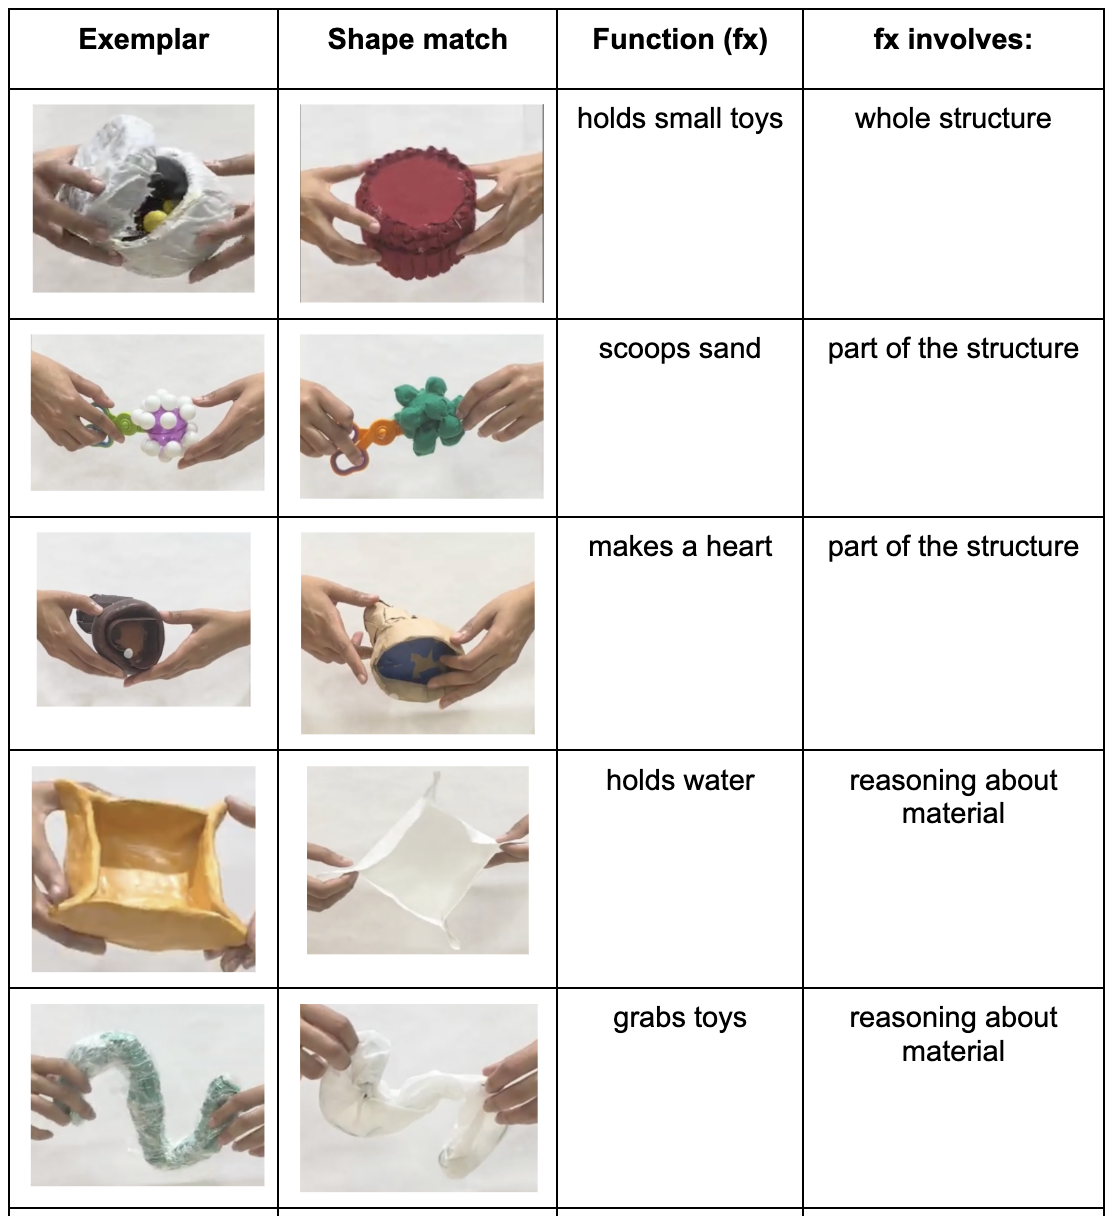
\includegraphics[width=1\linewidth]{stimuli} \caption[A diagram to visualize different factors that potentially contribute to the emergence of the shape bias]{A diagram to visualize different factors that potentially contribute to the emergence of the shape bias}\label{fig:stimulipics }
\end{figure}
\end{CodeChunk}

The function test object was modified in a way that preserved its shape
but altered its functionality (e.g., an object wrapped entirely vs.~one
that could clearly open). Color was excluded across all objects to
ensure that visual similarity was driven solely by shape, material, and
functional cues. Objects were crafted to explore how children reason
about similarity based on whole-object vs.~part-based features (e.g.,
whether specific parts afford a function). Some objects, such as the
``fep,'' ``blint,'' and ``wap,'' were designed with material-critical
functions (e.g., holding water while made of a paper towel). This design
tested whether children could prioritize material when reasoning about
function and to capture the developmental changes. The degree to which
object affordances were visually apparent varied across designs. For
example,the ``zimbo'' was designed to afford functionality only through
a specific part, while the overall structure was irrelevant. The
``gorp'' was modeled to resemble objects familiar to slightly older
children, like scissors, allowing exploration of prior experiences'
influence on categorization.

\subsubsection{Procedure}\label{procedure}

On each trial, the child was shown an object, which was labeled with the
phrase ``this is a {[}X{]}''. The object was moved away from the child
remained in view, and both test objects and the distractor were
displayed simultaneously while asking the child ``can you find another
{[}X{]} by pointing to it?''. The child gets to hear the label 3 times
while viewing it without touching it. Each child saw seven trials.

\begin{CodeChunk}
\begin{figure}[tb]
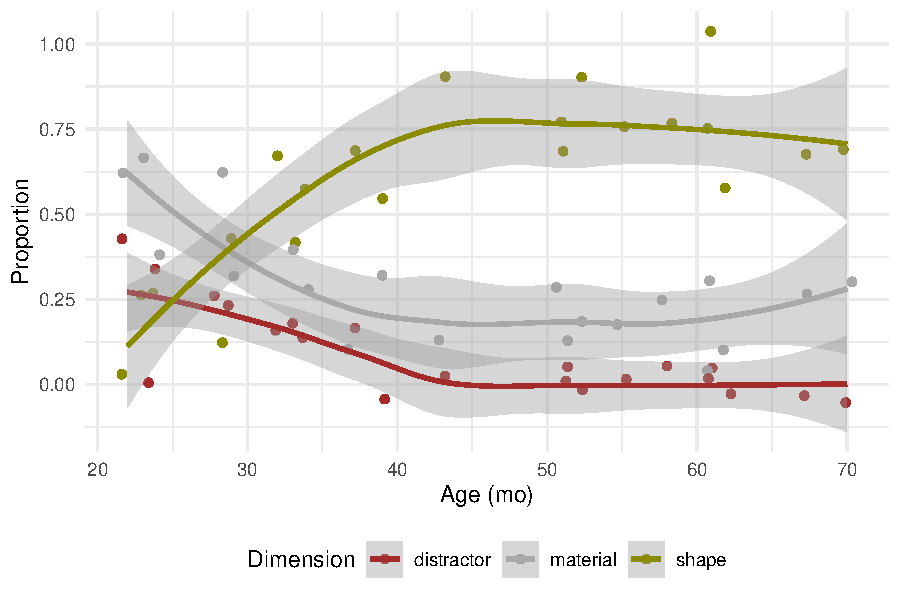
\includegraphics[width=1\linewidth]{figs/first_exp-1} \caption[Developmental trend of choosing by each dimension]{Developmental trend of choosing by each dimension. Smoothed lines are standard error}\label{fig:first_exp}
\end{figure}
\end{CodeChunk}

\begin{CodeChunk}
\begin{figure}[tb]
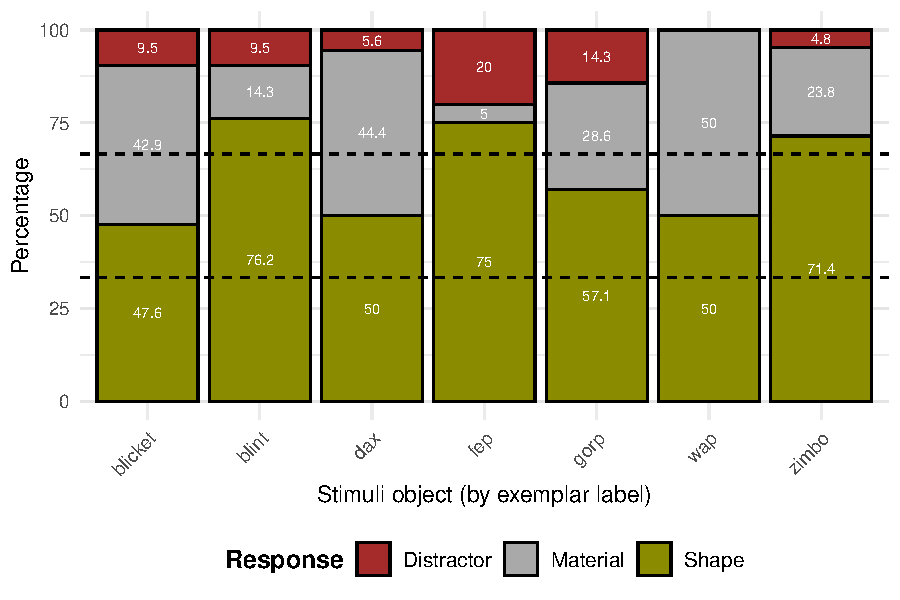
\includegraphics[width=1\linewidth]{figs/first_exp_stim-1} \caption[Percentage of choosing by dimension per stimuli item]{Percentage of choosing by dimension per stimuli item. Dashed line is chance level = 33.3\% }\label{fig:first_exp_stim}
\end{figure}
\end{CodeChunk}

\subsection{Results}\label{results}

Participants showed an overall shape bias across all trials (shape:
61\%, material: 30\%, distractor: 9\%). Figure \ref{fig:first_exp} shows
a developmental shift to choose by shape by age 3, replicating what is
seen previously in the literature.

To quantify these trends, we fit a generalized logistic mixed effects
model predicting the binary outcome of choosing by shape for each trial
by each child. We included random intercepts at the level of both
participants and stimuli objects. The average intercept odds of choosing
by shape were 0.11 (odds of 0.11:1 at the mean age, \(p=\) \textless{}
.001), with a significant increase in odds of 1.06 per unit increase in
age (\(p=\) \textless{} .001). The model also shows variability at the
item-level intercept (variance = 0.11, SD = 0.32) across 7 unique items
(standardlabel groups).

\subsection{Results and discussion}\label{results-and-discussion}

Even in a small sample of children between 2 and 5 years of age, data
from this experiment confirmed the robustness of the shape bias.
Although the reason why the younger group of kids i.e.~below 3, chose
more by material is not clear now, however, we see variability at the
item level such that for three objects ``blicket, dax, and wap'' we see
an above chance material choices when collapsing across ages. After
replicating the shape bias effect using the set of stimuli we created in
a simple set up, our next experiment explores a design that tests for
two conditions. The first is when shape is only contrasted with material
without any additional information. The second is a condition in which
shape is contrasted with function after demonstrating the function for
the exemplar, while controlling for individual differences with a bigger
sample size to capture variability at the item level as well as any
potential individual differences.

\section{Experiment 2}\label{experiment-2}

\subsection{Methods}\label{methods-1}

\subsubsection{Participants}\label{participants-1}

31 (target n=96, 24 per each age group) participants between 2-5 years
old (mean=48.22, SD=5.54, n per age group) were recruited from a local
nursery school in the US.

\subsubsection{Procedure}\label{procedure-1}

A within subject manipulation with two conditions: material or function.
The material condition is identical to the first experiment. In the
function condition, the experimenter introduce the exemplar object
``this is a dax'', gives the child 15 seconds seconds to play with it,
provides functional information `` the dax grapes toys'', gives another
15 seconds to play with it, and puts the toy away but within view,
before introducing the test objects and asks for a response.

\begin{CodeChunk}
\begin{figure*}[!h]
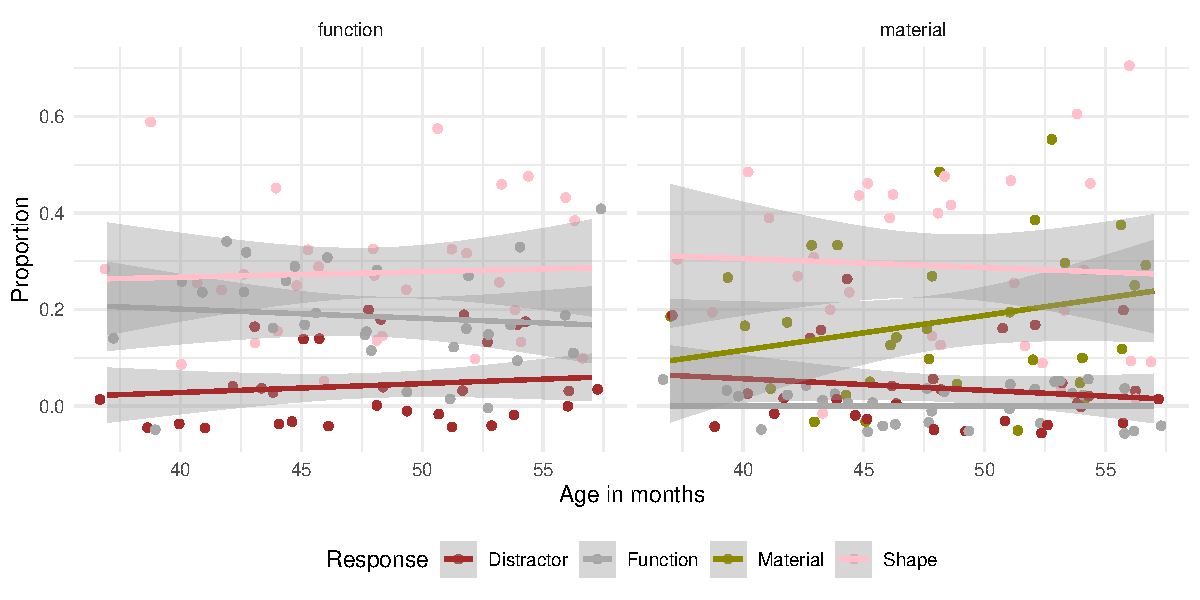
\includegraphics[width=1\linewidth]{figs/jitter_function-1} \caption[Experiment 2, function vs]{Experiment 2, function vs. no function 'material'  condition. Children choose by shape more, even when function information is made salient}\label{fig:jitter_function}
\end{figure*}
\end{CodeChunk}

\begin{CodeChunk}
\begin{figure}[tb]
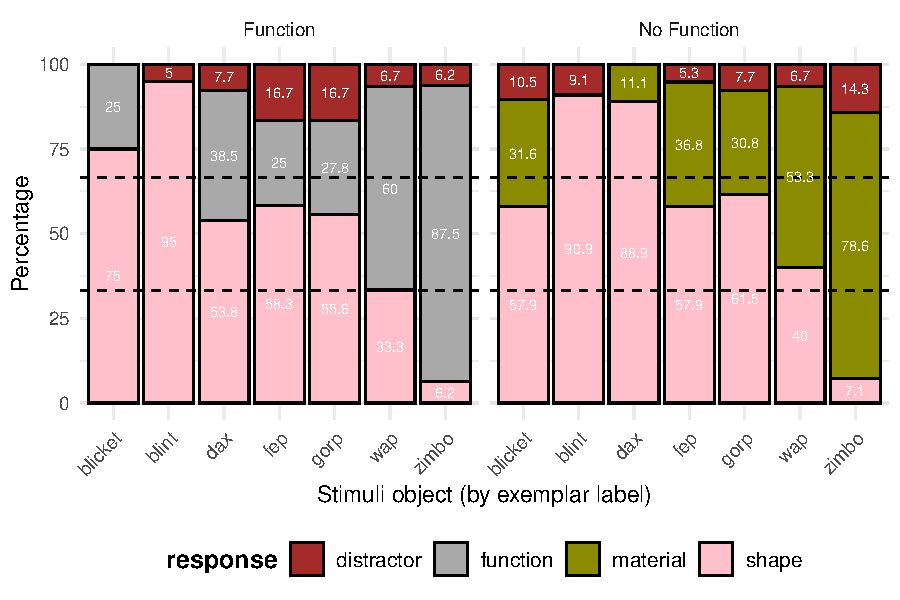
\includegraphics[width=1\linewidth]{figs/sec_exp_stim-1} \caption[Experiment 2, proportion of choosing by each dimension per exemplar item 'indicated by its novel label]{Experiment 2, proportion of choosing by each dimension per exemplar item 'indicated by its novel label. We note variability across items}\label{fig:sec_exp_stim}
\end{figure}
\end{CodeChunk}

\subsection{Preliminary results and
discussion}\label{preliminary-results-and-discussion}

Similar to what is conveyed in Figure \ref{fig:jitter_function}, a
generalized logistic mixed-effects model (GLMM) showed a lower baseline
odds of the shape bias in the material condition compared to the
function, and the odds ratio increases with age. In additon, random
effects indicate variability in intercepts across participants (SD =
0.22) and across items (SD = 1.38) for 31 participants and 7 items as in
Figure \ref{fig:sec_exp_stim}. (Notably, the confidence intervals show
uncertainty ``include 0'', however data collection is still ongoing.)

\subsection{General Discussion}\label{general-discussion}

The word extension and category organization literature is highly
heterogeneous. Studies in this domain lack an integrative and
commensurable design, which hinders our ability to draw consistent
conclusions. To achieve a more accurate measurement of category
organization and concept learning, we need a reliable and valid range
set of stimuli objects, consistent task formats and test designs, as
well as multi-site cross-cultural experiments unified across
laboratories to maximally account for the variability. Our evaluation of
the word extension literature reveals that making procedural decisions,
which we think are likely a primary source of unexplained variability,
is unattianable without running a series of controlled experiments that
would allow us to systematically assess how different designs and
stimuli covary with response patterns.

In our preliminary results, we see a tendency to generalize by shape,
even in conditions designed to make function salient. This suggests
that, even with a potential saliency effect, where the trials
highlighted functional information, it failed to override the preference
for shape-based choices. In addition, many children explored whether
their chosen test object could perform the intended function after
selecting it based on shape. This behavior implies that the shape-based
selection might not reflect a disregard for functional information but
rather a hypothesis that objects sharing shape might also share
functionality (for example, in the case of the dax, which is a box with
lid that you can use to store small toys, kids choose another box that
is wrapped all over to indicate impossibilty to open, and they still try
to open it afterwards). Meanwhile, in the case of the (gorp), for which
the function wasn't as ambiguous (scooping sand requires the structure
of the object to have two parts that can split and then close to hold
sand inside), in this case the test object was designed in a way that
makes it very clear to not open, hence they went for the function test
choice (see suplementary material). For evaulating the children's
ability to reason about intrinsic affordances, we created the ``Fep'' in
a way such that the material itself is very critical for performing the
function ``holding water while being made of paper towel''. We believe
all these structural differences between objects can explain part of the
variation when we have enough data to fit the model.

As we mentioned in the introduction, procedural variation observed in
the literature have followed theoretical debates and in fact reinforced
by them. We think this endeavor is one step towards achieving validity
and reliability in word extension tasks, as well as discussing
theoretical implications that follow for them. To illusatrate, the
definition of the shape bias construct as a word extension strategy has
been ambiguous and it is also influenced by theoretical framing. For
example, if it is a product of different contingencies and statistical
regularities, it would make sense from a signal detection point of view,
to predict that it will have a graded degree between population,
individuals, and items. Hence, analyzing data on an aggregate level
across all these dimensions hasn't helped advancing our understanding of
cross cultural differences at a theoretical level. We believe, providing
a quantifiable assessment of data across items, individuals, and
building upon that across cultures, will be the only way to resolve
these issues.

\section{References}\label{references}

\setlength{\parindent}{-0.1in} 
\setlength{\leftskip}{0.125in}

\noindent

\phantomsection\label{refs}
\begin{CSLReferences}{1}{0}
\bibitem[\citeproctext]{ref-abdelrahim_frank_2024}
Abdelrahim, S., \& Frank, M. C. (2024, September). Examining the
robustness and generalizability of the shape bias: A meta-analysis.
PsyArXiv.
http://doi.org/\href{https://doi.org/10.31234/osf.io/3by54}{10.31234/osf.io/3by54}

\bibitem[\citeproctext]{ref-BOOTH2002B11}
Booth, A. E., \& Waxman, S. R. (2002). Word learning is {``smart''}:
Evidence that conceptual information affects preschoolers' extension of
novel words. \emph{Cognition}, \emph{84}(1), B11--B22.
http://doi.org/\url{https://doi.org/10.1016/S0010-0277(02)00015-X}

\bibitem[\citeproctext]{ref-dejavu}
Booth, A., \& Waxman, S. (2006). Déjà vu all over again: Re-revisiting
the conceptual status of early word learning: Comment on smith and
samuelson (2006). \emph{Developmental Psychology}, \emph{42}, 1344--6.
http://doi.org/\href{https://doi.org/10.1037/0012-1649.42.6.1344}{10.1037/0012-1649.42.6.1344}

\bibitem[\citeproctext]{ref-2005_Booth}
Booth, A., Waxman, S., \& Huang, Y. (2005). Conceptual information
permeates word learning in infancy. \emph{Developmental Psychology},
\emph{41}(3), 491--505.
http://doi.org/\href{https://doi.org/10.1037/0012-1649.41.3.491}{10.1037/0012-1649.41.3.491}

\bibitem[\citeproctext]{ref-Bruner1964TheCO}
Bruner, J. S. (1964). The course of cognitive growth. \emph{American
Psychologist}, \emph{19}, 1--15. Retrieved from
\url{https://api.semanticscholar.org/CorpusID:145196722}

\bibitem[\citeproctext]{ref-Centner2003OnRM}
Centner, D. (2003). On relational meaning : The acquisition of verb
meaning. In. Retrieved from
\url{https://api.semanticscholar.org/CorpusID:7539638}

\bibitem[\citeproctext]{ref-cimpian2005absence}
Cimpian, A., \& Markman, E. M. (2005). The absence of a shape bias in
children's word learning. \emph{Developmental Psychology}, \emph{41}(6),
1003.

\bibitem[\citeproctext]{ref-colunga2000learning}
Colunga, E., \& Smith, L. B. (2000). Learning to learn words: A
cross-linguistic study of the shape and material biases. In
\emph{Proceedings of the 24th annual boston university conference on
language development} (Vol. 1, pp. 197--207).

\bibitem[\citeproctext]{ref-gathercole_1997}
Gathercole, V. C. M., \& Min, H. (1997). Word meaning biases or
language-specific effects? {Evidence} from {English}, {Spanish} and
{Korean}. \emph{First Language}, \emph{17}(51), 031--56.
http://doi.org/\href{https://doi.org/10.1177/014272379701705102}{10.1177/014272379701705102}

\bibitem[\citeproctext]{ref-gershkoff2004shape}
Gershkoff-Stowe, L., \& Smith, L. B. (2004). Shape and the first hundred
nouns. \emph{Child Development}, \emph{75}(4), 1098--1114.

\bibitem[\citeproctext]{ref-GRAHAM1999128}
Graham, S. A., Williams, L. D., \& Huber, J. F. (1999). Preschoolers'
and adults' reliance on object shape and object function for lexical
extension. \emph{Journal of Experimental Child Psychology},
\emph{74}(2), 128--151.
http://doi.org/\url{https://doi.org/10.1006/jecp.1999.2514}

\bibitem[\citeproctext]{ref-imai1997}
Imai, M., \& Gentner, D. (1997). A cross-linguistic study of early word
meaning: Universal ontology and linguistic influence. \emph{Cognition},
\emph{62}(2), 169--200.

\bibitem[\citeproctext]{ref-jara2022}
Jara-Ettinger, J., Levy, R., Sakel, J., Huanca, T., \& Gibson, E.
(2022). The origins of the shape bias: Evidence from the tsimane'.
\emph{Journal of Experimental Psychology: General}.

\bibitem[\citeproctext]{ref-Jones2003}
Jones, Susan S. (2003). Late talkers show no shape bias in a novel name
extension task. \emph{Developmental Science}, \emph{6}(5), 477--483.
http://doi.org/\url{https://doi.org/10.1111/1467-7687.00304}

\bibitem[\citeproctext]{ref-JONES1993113}
Jones, Susan S., \& Smith, L. B. (1993). The place of perception in
children's concepts. \emph{Cognitive Development}, \emph{8}(2),
113--139.
http://doi.org/\url{https://doi.org/10.1016/0885-2014(93)90008-S}

\bibitem[\citeproctext]{ref-JONES1998323}
Jones, Susan S., \& Smith, L. B. (1998). How children name objects with
shoes. \emph{Cognitive Development}, \emph{13}(3), 323--334.
http://doi.org/\url{https://doi.org/10.1016/S0885-2014(98)90014-4}

\bibitem[\citeproctext]{ref-JONES_SMITH_2005}
JONES, S. S., \& SMITH, L. B. (2005). Object name learning and object
perception: A deficit in late talkers. \emph{Journal of Child Language},
\emph{32}(1), 223--240.
http://doi.org/\href{https://doi.org/10.1017/S0305000904006646}{10.1017/S0305000904006646}

\bibitem[\citeproctext]{ref-Kucker2019ReproducibilityAA}
Kucker, S. C., Samuelson, L. K., Perry, L. K., Yoshida, H., Colunga, E.,
Lorenz, M. G., \& Smith, L. B. (2019). Reproducibility and a unifying
explanation: Lessons from the shape bias. \emph{Infant Behavior \&
Development}, \emph{54}, 156--165. Retrieved from
\url{https://api.semanticscholar.org/CorpusID:53045726}

\bibitem[\citeproctext]{ref-landau1996}
Landau, B., \& Jones, S. (1998). Object shape, object function, and
object name. \emph{Journal of Memory and Language - J MEM LANG},
\emph{38}, 1--27.
http://doi.org/\href{https://doi.org/10.1006/jmla.1997.2533}{10.1006/jmla.1997.2533}

\bibitem[\citeproctext]{ref-LANDAU1988299}
Landau, B., Smith, L. B., \& Jones, S. S. (1988). The importance of
shape in early lexical learning. \emph{Cognitive Development},
\emph{3}(3), 299--321.
http://doi.org/\url{https://doi.org/10.1016/0885-2014(88)90014-7}

\bibitem[\citeproctext]{ref-Merriman_Scott_Marazita_1993}
Merriman, W. E., Scott, P. D., \& Marazita, J. (1993). An
appearance-function shift in children's object naming. \emph{Journal of
Child Language}, \emph{20}(1), 101--118.
http://doi.org/\href{https://doi.org/10.1017/S0305000900009144}{10.1017/S0305000900009144}

\bibitem[\citeproctext]{ref-perry2010learn}
Perry, L. K., Samuelson, L. K., Malloy, L. M., \& Schiffer, R. N.
(2010). Learn locally, think globally: Exemplar variability supports
higher-order generalization and word learning. \emph{Psychological
Science}, \emph{21}(12), 1894--1902.

\bibitem[\citeproctext]{ref-samuelson_statistical_2002}
Samuelson, Larissa K. (2002). Statistical regularities in vocabulary
guide language acquisition in connectionist models and 15-20-month-olds.
\emph{Developmental Psychology}, \emph{38}(6), 1016--1037.
http://doi.org/\href{https://doi.org/10.1037/0012-1649.38.6.1016}{10.1037/0012-1649.38.6.1016}

\bibitem[\citeproctext]{ref-2005_Samuelson}
Samuelson, Larissa K. (2005). Statistical regularities in vocabulary
guide language acquisition in connectionist models and 15-20-month-olds.
\emph{Developmental Psychology}, \emph{38}(6), 1016--1037.
http://doi.org/\href{https://doi.org/10.1037/0012-1649.38.6.1016}{10.1037/0012-1649.38.6.1016}

\bibitem[\citeproctext]{ref-samuelson2008rigid}
Samuelson, Larissa K., Horst, J. S., Schutte, A. R., \& Dobbertin, B. N.
(2008). Rigid thinking about deformables: Do children sometimes
overgeneralize the shape bias? \emph{Journal of Child Language},
\emph{35}(3), 559--589.

\bibitem[\citeproctext]{ref-SAMUELSON2010138}
Samuelson, Larissa K., \& Perone, S. (2010). Rethinking
conceptually-based inference --- grounding representation in task and
behavioral dynamics: Commentary on {``fifteen-month-old infants attend
to shape over other perceptual properties in an induction task,''} by s.
Graham and g. Diesendruck, and {``form follows function: Learning about
function helps children learn about shape,''} by e. Ware and a. booth.
\emph{Cognitive Development}, \emph{25}(2), 138--148.
http://doi.org/\url{https://doi.org/10.1016/j.cogdev.2010.02.002}

\bibitem[\citeproctext]{ref-samuelson1999}
Samuelson, Larissa K., \& Smith, L. B. (1999). Early noun vocabularies:
Do ontology, category structure and syntax correspond? \emph{Cognition},
\emph{73}(1), 1--33.

\bibitem[\citeproctext]{ref-dynamicBias}
Samuelson, L., \& Horst, J. (2008). Shape bias special section:
Confronting complexity: Insights from the details of behavior over
multiple timescales. \emph{Developmental Science}, \emph{11}, 209--15.
http://doi.org/\href{https://doi.org/10.1111/j.1467-7687.2007.00667.x}{10.1111/j.1467-7687.2007.00667.x}

\bibitem[\citeproctext]{ref-Smith2003MakingAO}
Smith, L. B., Colunga, E., \& Yoshida, H. (2003). Making an ontology:
Cross-linguistic evidence. In. Retrieved from
\url{https://api.semanticscholar.org/CorpusID:195941919}

\bibitem[\citeproctext]{ref-smithcolunga2010}
Smith, L. B., Colunga, E., \& Yoshida, H. (2010). Knowledge as process:
Contextually cued attention and early word learning. \emph{Cognitive
Science}, \emph{34}(7), 1287--1314.
http://doi.org/\url{https://doi.org/10.1111/j.1551-6709.2010.01130.x}

\bibitem[\citeproctext]{ref-Smith1996NamingIY}
Smith, L. B., Jones, S. S., \& Landau, B. (1996). Naming in young
children: A dumb attentional mechanism? \emph{Cognition}, \emph{60},
143--171. Retrieved from
\url{https://api.semanticscholar.org/CorpusID:18659784}

\bibitem[\citeproctext]{ref-smith_object_2002}
Smith, L. B., Jones, S. S., Landau, B., Gershkoff-Stowe, L., \&
Samuelson, L. (2002). Object name learning provides on-the-job training
for attention. \emph{Psychological Science}, \emph{13}(1), 13--19.
http://doi.org/\href{https://doi.org/10.1111/1467-9280.00403}{10.1111/1467-9280.00403}

\bibitem[\citeproctext]{ref-soja1991ontological}
Soja, Nancy N., Carey, S., \& Spelke, E. S. (1991). Ontological
categories guide young children's inductions of word meaning: Object
terms and substance terms. \emph{Cognition}, \emph{38}(2), 179--211.

\bibitem[\citeproctext]{ref-soja_perception_1992}
Soja, Nancy N., Carey, S., \& Spelke, E. S. (1992). Perception,
ontology, and word meaning. \emph{Cognition}, \emph{45}(1), 101--107.
http://doi.org/\href{https://doi.org/10.1016/0010-0277(92)90025-D}{10.1016/0010-0277(92)90025-D}

\bibitem[\citeproctext]{ref-subrahmanyam_2006}
Subrahmanyam, K., \& Chen, H.-H. N. (2006). A crosslinguistic study of
children's noun learning: {The} case of object and substance words.
\emph{First Language}, \emph{26}(2), 141--160.
http://doi.org/\href{https://doi.org/10.1177/0142723706060744}{10.1177/0142723706060744}

\bibitem[\citeproctext]{ref-TekAutism}
Tek, S., Jaffery, R., Fein, D., \& Naigles, L. (2008). Do children with
autism show a shape bias in word learning? \emph{Autism Research :
Official Journal of the International Society for Autism Research},
\emph{1}, 208--22.
http://doi.org/\href{https://doi.org/10.1002/aur.38}{10.1002/aur.38}

\bibitem[\citeproctext]{ref-TekAutismLessons}
Tek, S., \& Naigles, L. (2017). The shape bias as a word-learning
principle: Lessons from and for autism spectrum disorder.
\emph{Translational Issues in Psychological Science}, \emph{3}, 94--103.
http://doi.org/\href{https://doi.org/10.1037/tps0000104}{10.1037/tps0000104}

\bibitem[\citeproctext]{ref-WARE2010124}
Ware, E. A., \& Booth, A. E. (2010). Form follows function: Learning
about function helps children learn about shape. \emph{Cognitive
Development}, \emph{25}(2), 124--137.
http://doi.org/\url{https://doi.org/10.1016/j.cogdev.2009.10.003}

\bibitem[\citeproctext]{ref-yoshida2003known}
Yoshida, H., \& Smith, L. B. (2003a). Known and novel noun extensions:
Attention at two levels of abstraction. \emph{Child Development},
\emph{74}(2), 564--577.

\bibitem[\citeproctext]{ref-yoshida2003}
Yoshida, H., \& Smith, L. B. (2003b). Shifting ontological boundaries:
How japanese- and english-speaking children generalize names for animals
and artifacts. \emph{Developmental Science}, \emph{6}(1), 1--17.
http://doi.org/\url{https://doi.org/10.1111/1467-7687.00247/_1}

\end{CSLReferences}

\bibliographystyle{apacite}


\end{document}
